\chapter{Cài đặt thử nghiệm}

\section{Môi trường và cách triển khai}

Hệ thống được đóng gói và triển khai bằng Docker Compose với 5 container (Chương 6, Bảng~\ref{tab:components}). Lần đầu khởi động, container \texttt{api} tự chạy migration (\texttt{db/migrations/001\_init.sql}) và nạp dữ liệu mẫu bám theo quy trình (11 đơn vị, 5 vai trò, 6 thiết bị mẫu theo định nghĩa 5.1 của quy trình, kế hoạch năm 2026, sự cố, biên bản nghiệm thu).

\begin{verbatim}
# Khởi động toàn bộ hệ thống
docker compose up -d --build

# Cổng đơn vị sử dụng :  http://localhost:8080
# Cổng quản trị       :  http://localhost:8081
# API                 :  http://localhost:3001/api/v1/health
\end{verbatim}

\section{Kết quả thử nghiệm các luồng nghiệp vụ}

Hệ thống được thử nghiệm end-to-end qua API và giao diện. Kết quả:

\begin{table}[h]
\centering
\caption{Kết quả thử nghiệm các kịch bản chính}
\label{tab:test}
\begin{tabular}{P{0.8cm}P{8.6cm}P{3.2cm}P{2.2cm}}
\toprule
\textbf{STT} & \textbf{Kịch bản} & \textbf{Luồng kiểm chứng} & \textbf{Kết quả} \\
\midrule
1 & Đăng nhập 4 vai trò (đơn vị, Văn phòng Cục, Lãnh đạo Cục, QMS) & JWT trả về đúng vai trò; sai mật khẩu chặn 401 & Đạt \\
2 & Đơn vị báo sự cố nhỏ (máy in) & Mã SC-2026-xxx sinh tự động; thiết bị chuyển ``Sự cố''; VPC nhận thông báo & Đạt \\
3 & VPC xem xét, phân loại tự khắc phục; đơn vị tự khắc phục & Không qua phê duyệt; hồ sơ BM/02 tự thêm bản ghi; sự cố đóng; thiết bị về ``Hoạt động'' & Đạt \\
4 & Đơn vị báo sự cố lớn $\rightarrow$ VPC lập phương án thuê ngoài $\rightarrow$ Lãnh đạo Cục phê duyệt & Thiết bị chuyển ``Đang sửa chữa''; từ chối không ghi lý do bị chặn & Đạt \\
5 & Báo hoàn thành $\rightarrow$ lập biên bản BM/04 (2 bên đại diện) $\rightarrow$ ký đủ & Sự cố đóng; hồ sơ thiết bị thêm bản ghi ``Sửa chữa''; thiết bị về ``Hoạt động'' & Đạt \\
6 & Lập kế hoạch năm 2026 (4 hạng mục) $\rightarrow$ trình $\rightarrow$ phê duyệt & Trạng thái Nháp $\rightarrow$ Chờ duyệt $\rightarrow$ Đã duyệt; thông báo gửi đúng vai trò & Đạt \\
7 & Hoàn thành hạng mục bảo dưỡng theo kế hoạch & Tự ghi hồ sơ BM/02; thiết bị trả về ``Hoạt động'' & Đạt \\
8 & Xuất danh mục Excel (BM/01) & File .xlsx đúng 6 cột biểu mẫu & Đạt \\
9 & Phân quyền: đơn vị cố sửa thiết bị (403), QMS cố duyệt (403) & Middleware \texttt{requireRole} chặn đúng & Đạt \\
10 & Nhật ký thao tác & Mọi thao tác tạo/duyệt/ký/đăng nhập được ghi audit trail append-only & Đạt \\
\bottomrule
\end{tabular}
\end{table}

\section{Ảnh chụp màn hình hệ thống}

\begin{figure}[h]
\centering
\IfFileExists{figures/screen-admin-dashboard.png}{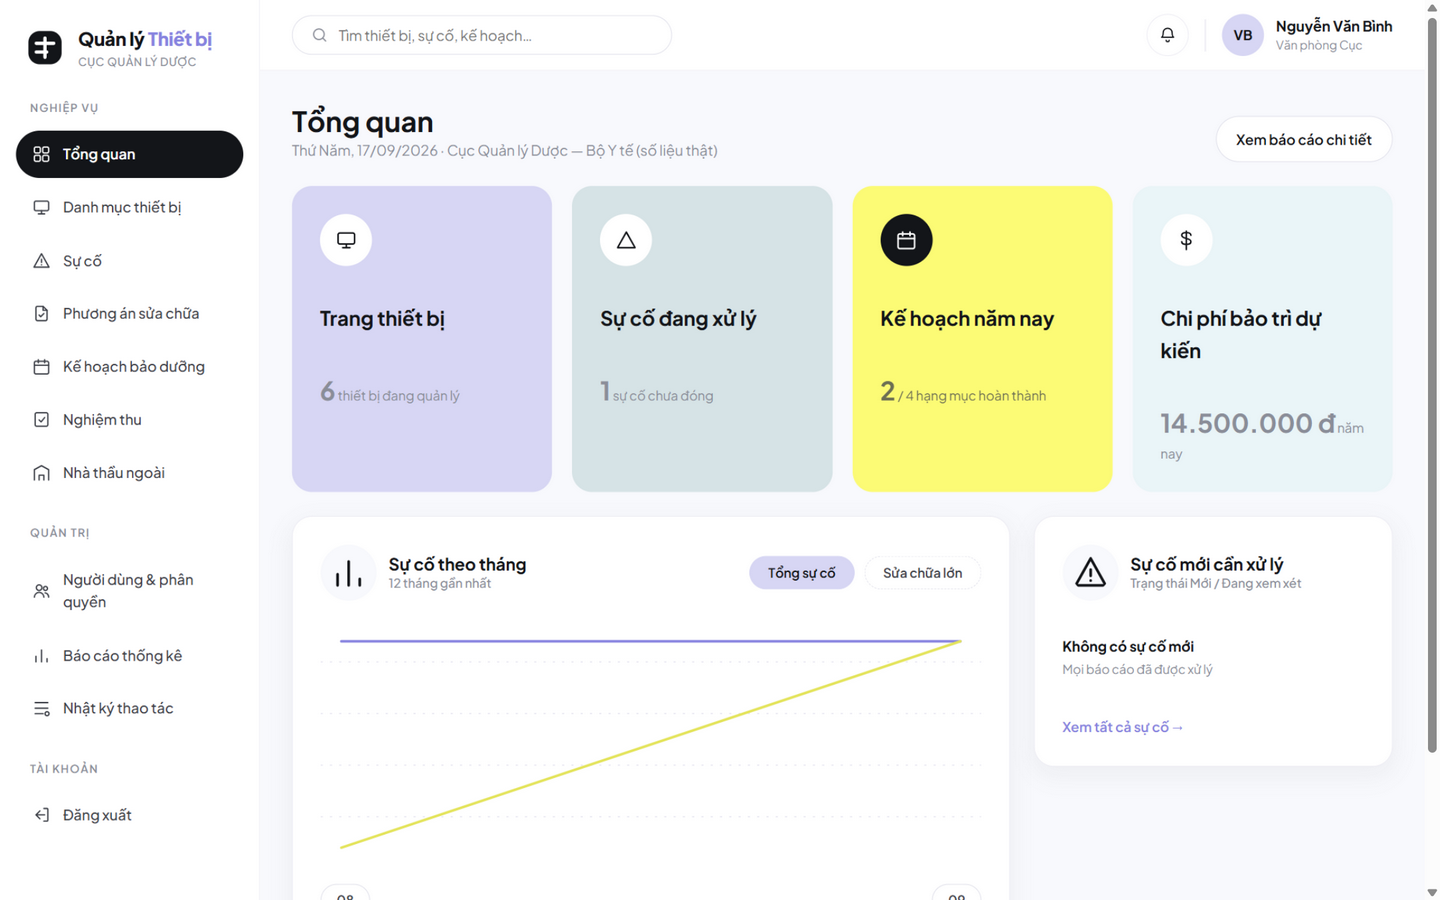
\includegraphics[width=\textwidth]{figures/screen-admin-dashboard.png}}{\fbox{\parbox{0.9\textwidth}{\centering Dashboard quản trị (xem demo trực tiếp tại cổng quản trị)}}}
\caption{Cổng quản trị — dashboard tổng quan với số liệu thật}
\label{fig:scr-dash}
\end{figure}

\begin{figure}[h]
\centering
\IfFileExists{figures/screen-user-home.png}{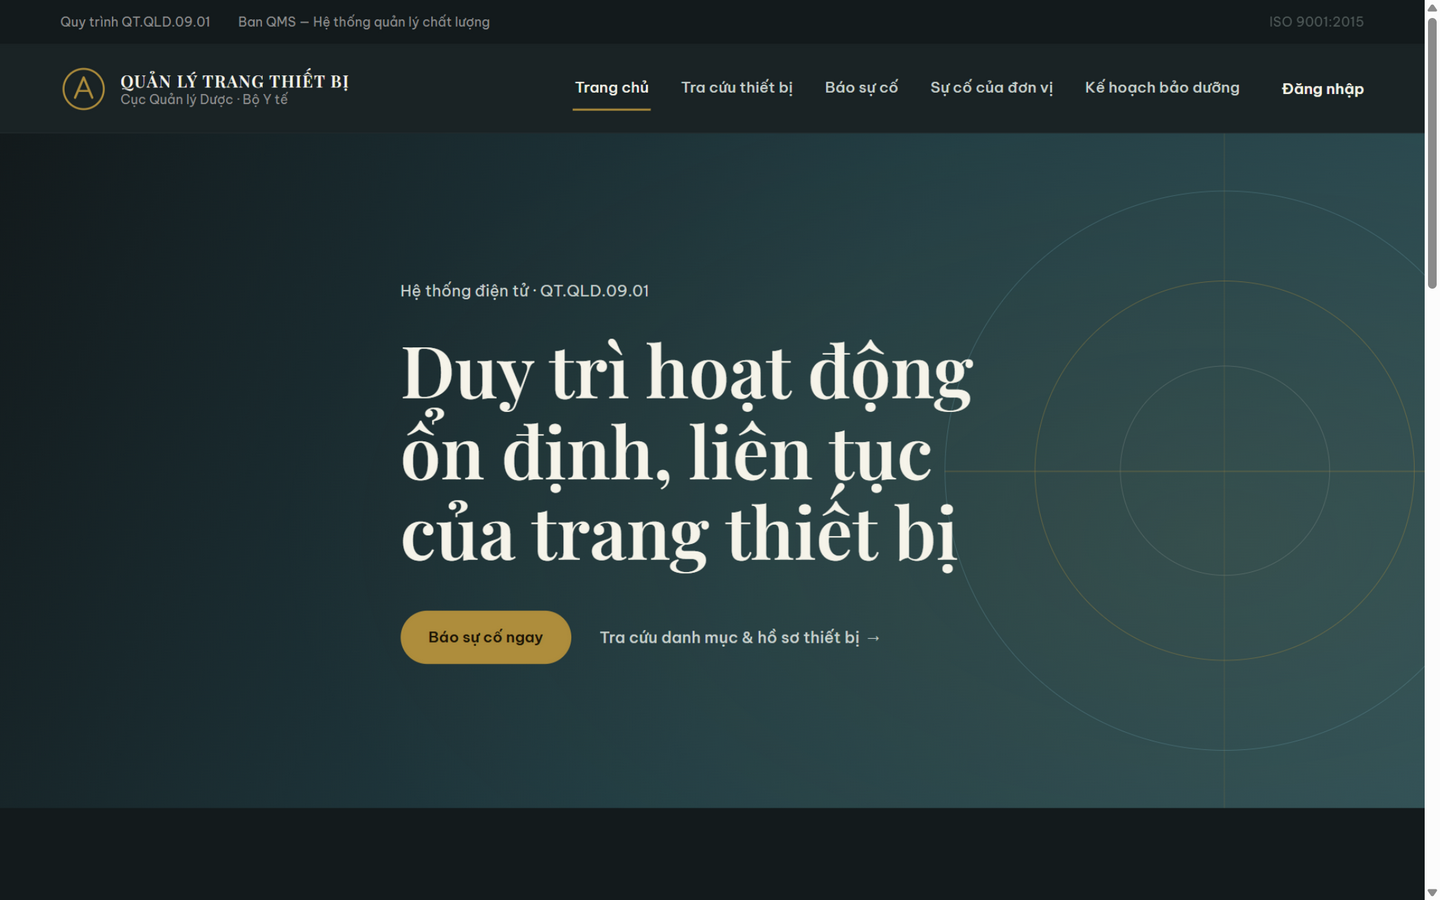
\includegraphics[width=\textwidth]{figures/screen-user-home.png}}{\fbox{\parbox{0.9\textwidth}{\centering Trang chủ cổng đơn vị sử dụng}}}
\caption{Cổng đơn vị sử dụng — trang chủ và tra cứu nhanh}
\label{fig:scr-home}
\end{figure}

\begin{figure}[h]
\centering
\IfFileExists{figures/screen-profile.png}{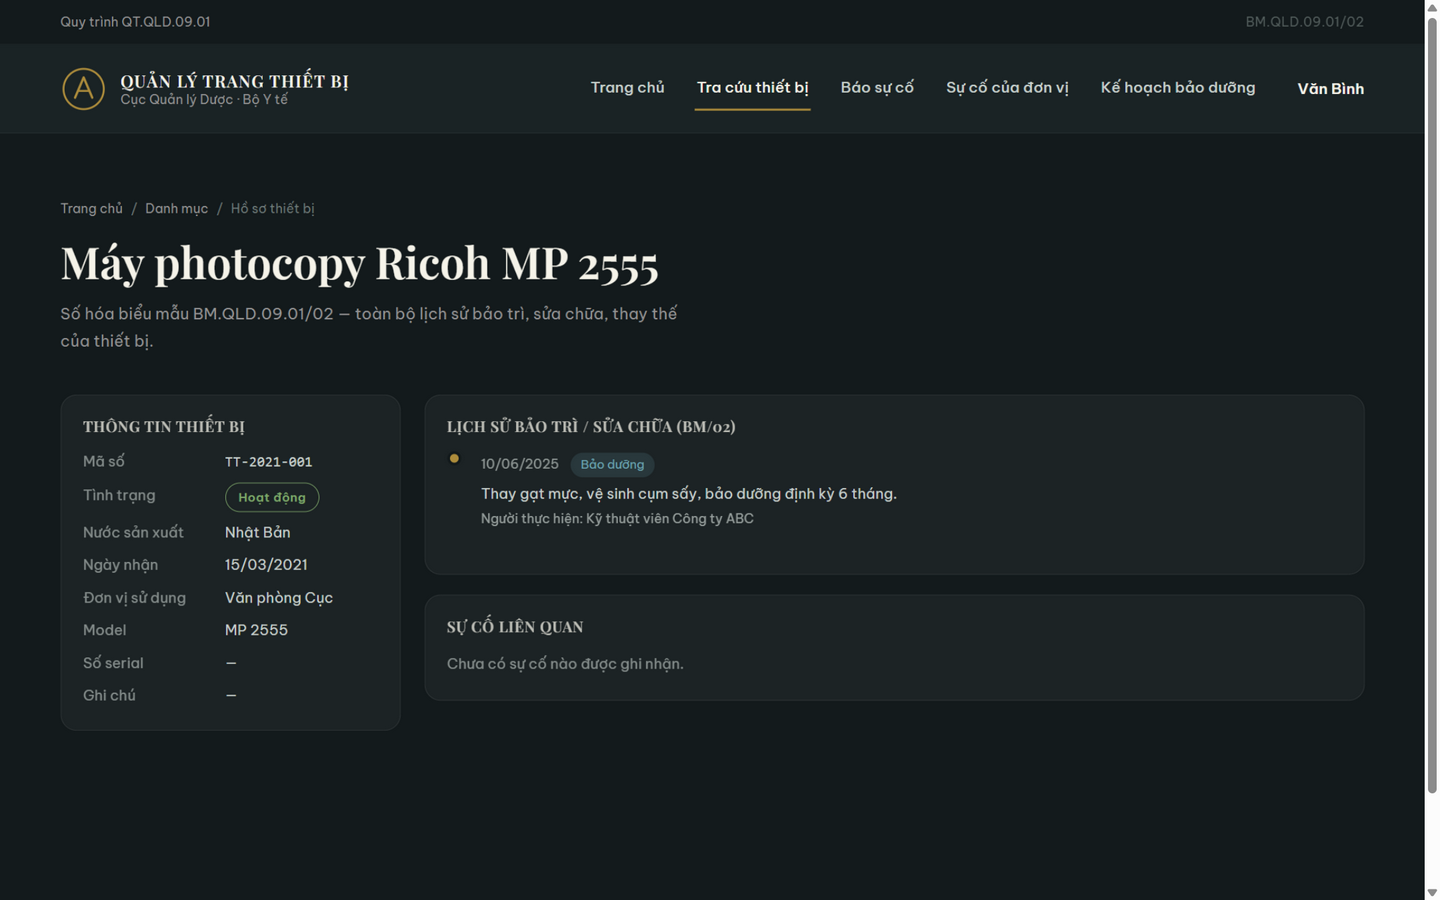
\includegraphics[width=\textwidth]{figures/screen-profile.png}}{\fbox{\parbox{0.9\textwidth}{\centering Hồ sơ thiết bị dạng timeline (BM/02)}}}
\caption{Hồ sơ trang thiết bị — timeline lịch sử bảo trì, sửa chữa}
\label{fig:scr-profile}
\end{figure}

\begin{figure}[h]
\centering
\IfFileExists{figures/screen-acceptance.png}{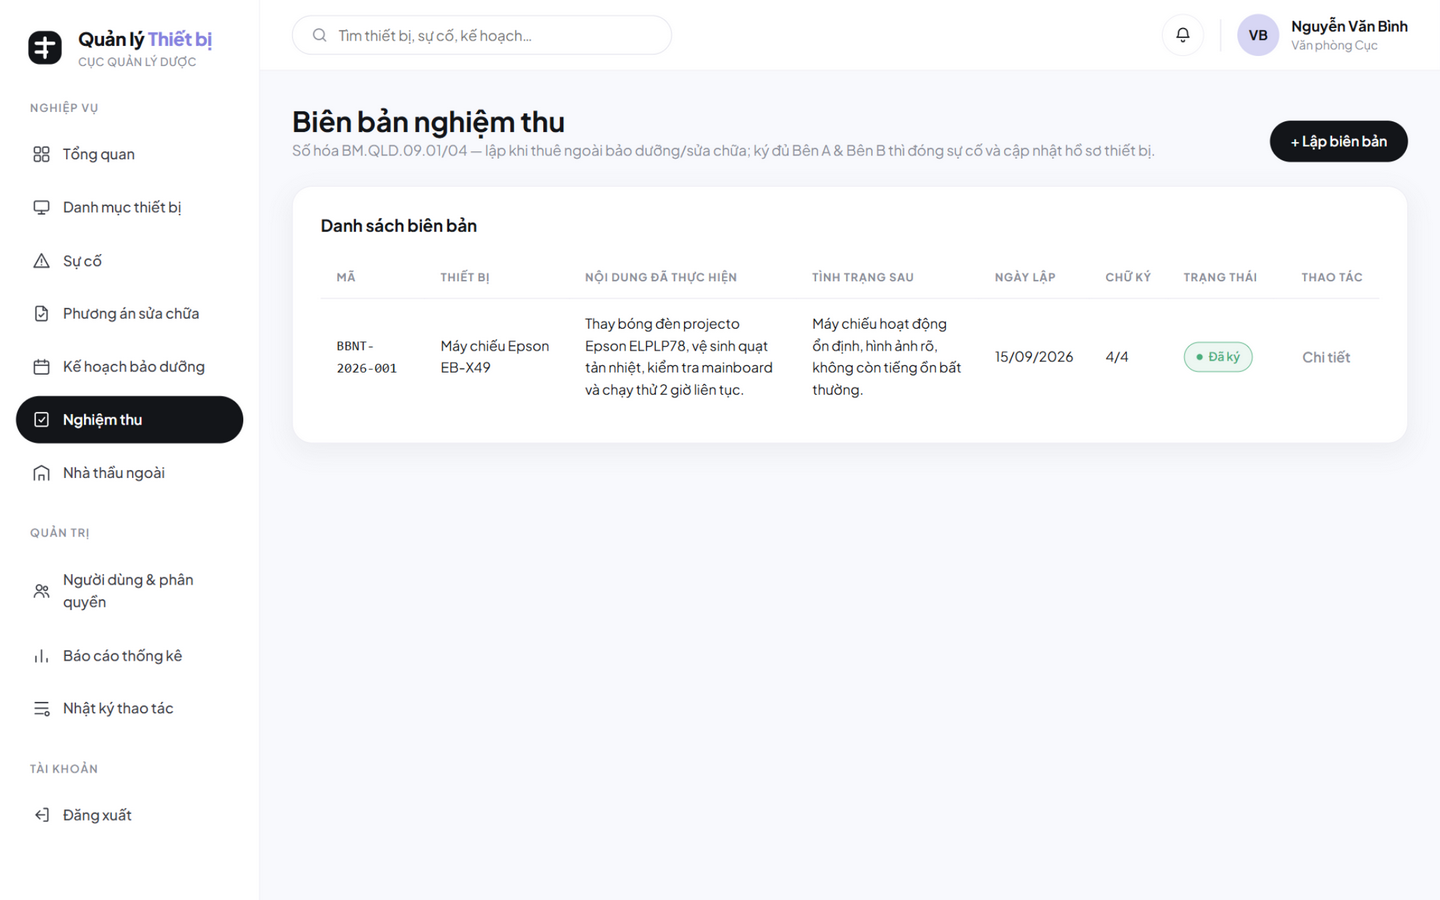
\includegraphics[width=\textwidth]{figures/screen-acceptance.png}}{\fbox{\parbox{0.9\textwidth}{\centering Danh sách biên bản nghiệm thu (BM/04)}}}
\caption{Nghiệm thu điện tử — theo dõi tiến độ ký của hai bên}
\label{fig:scr-acc}
\end{figure}

\section{Giới hạn của nguyên mẫu}

\begin{itemize}
  \item Chữ ký điện tử hiện là mô phỏng (ghi nhận tên + thời điểm), chưa tích hợp chữ ký số theo Nghị định 130/2020/NĐ-CP.
  \item Chưa chạy song song với biểu mẫu giấy trong môi trường thật; kịch bản chuyển đổi cần Ban QMS phê duyệt.
  \item Chưa đo lường chính thức hiệu năng và tải; chưa có bộ kiểm thử tự động hóa đầy đủ (hiện thử nghiệm thủ công theo Bảng~\ref{tab:test}).
\end{itemize}
